\subsection{Frequency Stability vs. Size, Weight, and Power (SWaP)}
\label{subsec:stability_vs_SWaP}

As we have seen in the previous paragraphs, a strong correlation exists between the stability of the clock and its size, weight, and power consumption.
To achieve better performances, a series of internal components must be increased in size (e.g. the reference cell) or quality (e.g. the local oscillator), or additional servo loops must be added to control the disturbances (and indeed more sensor and actuator are required).

So qualitatively, we can understand how better performances are associated with an increase in the SWaP of the clock.
In Figure \ref{fig:ADEV_vs_SWaP}, we can observe how the Allan deviation $\sigma_y(\tau=1s)$ is related to the SWaP of the clock for different types of atomic clocks, ranging from the traditional table-size atomic clock to the CSAC.

\begin{figure}[H]
    \centering
    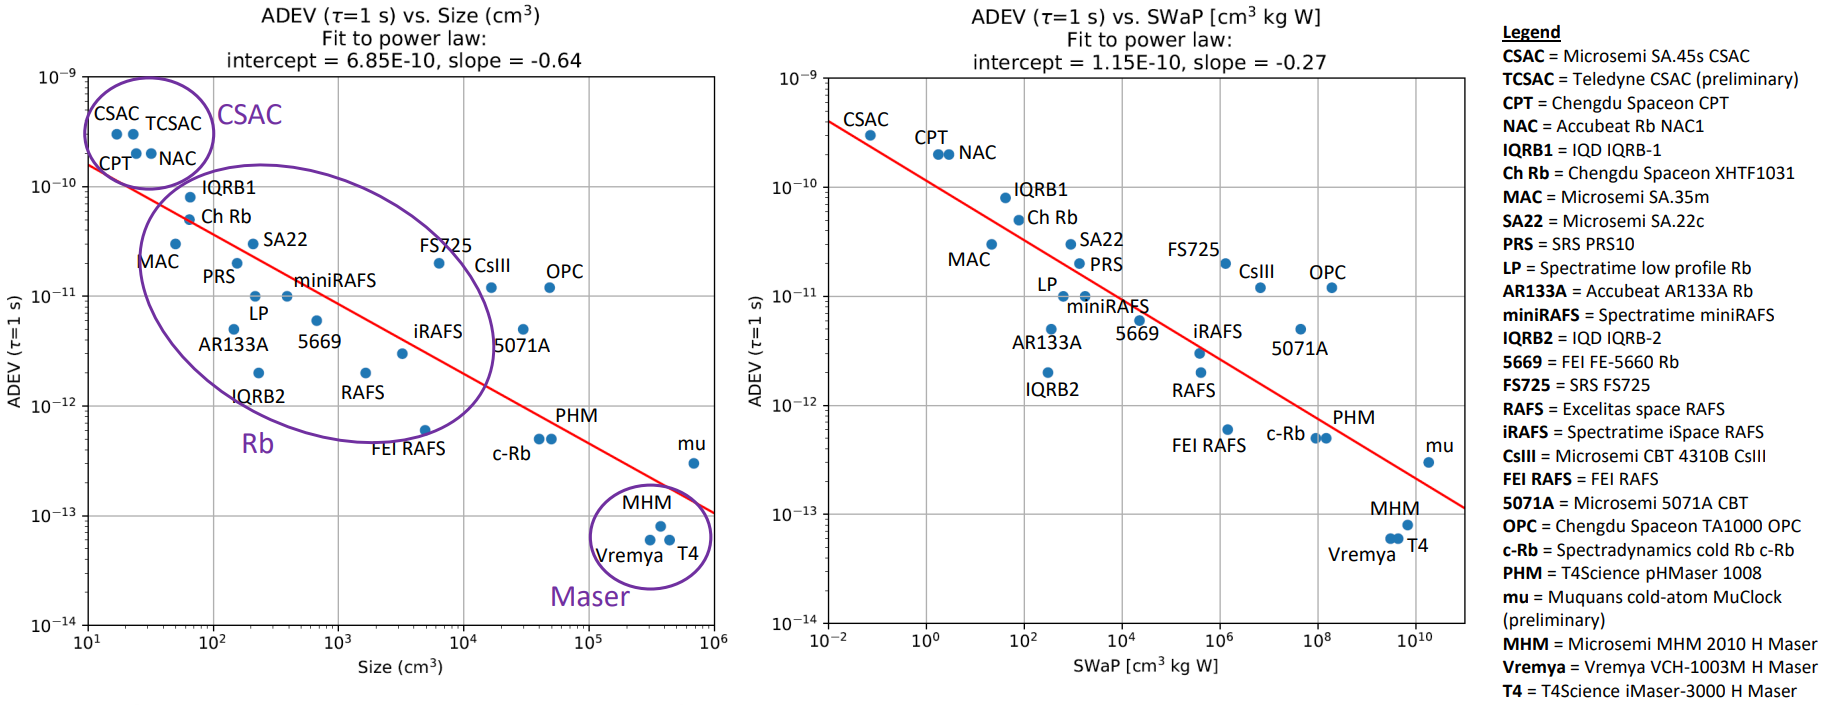
\includegraphics[width=\textwidth, max width=\linewidth]{img/ADEV_vs_SWaP.png}
    \caption{Allan deviation $\sigma_y(\tau=1s)$ vs. Size, Weight, and Power (SWaP) for different atomic clocks. Source \cite{Scherer}.}
    \label{fig:ADEV_vs_SWaP}
\end{figure}

As also marked by the red lines in both the plots, it's clear that a correlation exist and that is not possible to achieve a very high stability without a significant increase in the SWaP of the clock.
In particular, the equations of the two red lines are\footnote{The units adopted in the equations related to the SWaP are: Size and Volume $[cm^3]$, Weight $[kg]$, Power $[W]$}:

\begin{align}
    \sigma_y(\tau=1s) & = 6.85 \times 10^{-10} + \text{volume}^{-0.64} \\
    \sigma_y(\tau=1s) & = 1.15 \times 10^{-10} + \text{SWaP}^{-0.27}
\end{align}


